\chapter{涵道风扇式无人机的姿态控制}

基于第二章建立的DFUAV非线性系统动态方程分析,其多源力与力矩耦合叠加效应导致姿态动态模型尤为复杂。如滚转角的变化会在俯仰通道和偏航通道上都产生或者间接产生力矩影响,并且三维力矩都与环境风速呈现强相关性。最常用的姿态控制方法基于反馈线性化,比如不考虑系统的数学模型的PID控制算法,虽然该方法面对非线性系统有一定的鲁棒性,但仅通过比例-积分-微分的线性组合应对内外因素产生的力矩影响难免会使系统状态出现超调和滞后等问题。此外,可以使用基于系统模型的方法考虑内外因素对系统状态的影响,但在系统模型参数过多并且不精确的情况下也将为控制算法的设计和系统调试带来很大工作量。基于上述分析,姿态控制算法设计的核心在于如何对难以测得的力矩进行在线补偿。

本章安排如下:首先简要概述增量非线性动态逆控制和控制分配的理论以及二者的结合,然后对DFUAV的姿态动力学模型进行简化处理,方便下文姿态控制算法的设计。接下来给出了基于INDI和优先级控制分配的DFUAV的姿态控制方案设计,最后为验证方案有效性,最后进行了仿真实验和飞行实验验证。

\section{增量非线性动态逆控制与控制分配理论}

NDI(非线性动态逆)是一种基于模型的非线性控制方法,其核心在于在掌握系统模型的情况下,将非线性系统在工作点处进行反馈线性化,然后通过求逆运算来消除系统中的非线性项。当系统模型参数不精确或者对系统机理认识模糊的情况下,NDI方法的控制效果将表现不佳。而INDI(增量式非线性动态逆)相比于NDI采用了增量式的控制策略,仅要求对系统的输入通道建模。INDI在未能充分掌握系统模型的情况下,通过增量式的求逆策略来实时补偿未知扰动与建模误差,得到线性化的系统动力学,进而可以通过常规的线性系统的控制方法来控制\cite{wangStabilityAnalysisIncremental2019b}。因此INDI方法对系统模型的依赖程度较小,是一种基于传感器的方法。此外,INDI方法在设计控制律时主要关注系统的输入输出特性,无需考虑应如何将控制律计算出的控制量分配到各个执行机构上。而后者所描述的任务将由控制分配算法来实现,实现过程中也无需考虑系统内部的复杂非线性因素与动态干扰。因此,采用INDI控制方法有助于将姿态控制算法设计与控制分配算法分离开,实现分层控制。

本节首先将从一般性的系统推导INDI是如何实现增量控制的,然后介绍控制分配理论以及二者的结合。

\subsection{增量非线性动态逆}

考虑如下普通的非线性动力系统:
\begin{align}
    \dot{\boldsymbol{x}}&=\boldsymbol{f}(\boldsymbol{x})+\boldsymbol{g}(\boldsymbol{x},\boldsymbol{u}) \label{3-1}
    \\
    \boldsymbol{y}&=\boldsymbol{h}(\boldsymbol{x})\label{3-2}
\end{align}
上式中$\boldsymbol{x}\in\mathbb{R}^{n}$为n维系统状态变量,$\boldsymbol{u}\in\boldsymbol{U}\in\mathbb{R}^{p}$为p维系统输入变量,其中$\boldsymbol{U}$是容许控制集合,表示对输入变量的约束,$\boldsymbol{y}\in\mathbb{R}^{m}$为m维系统输出变量。映射关系$\boldsymbol{f}:\mathbb{R}^n\rightarrow\mathbb{R}^n$,$\boldsymbol{g}:\mathbb{R}^n\times\mathbb{R}^p\rightarrow\mathbb{R}^n$,$\boldsymbol{h}:\mathbb{R}^n\rightarrow\mathbb{R}^m$。

式\eqref{3-1}中系统状态的一阶泰勒展开式为:
\begin{equation}
    \dot{\boldsymbol{x}}=\dot{\boldsymbol{x}}_0+f^{\prime}(\boldsymbol{x})(\boldsymbol{x}-\boldsymbol{x}_0)+\left.\frac{\partial \boldsymbol{g}}{\partial \boldsymbol{x}}\right|_{\boldsymbol{x}=\boldsymbol{x}_0}(\boldsymbol{x}-\boldsymbol{x}_0)+\left.\frac{\partial \boldsymbol{g}}{\partial \boldsymbol{u}}\right|_{\boldsymbol{u}=\boldsymbol{u}_0}(\boldsymbol{u}-\boldsymbol{u}_0)
    \label{3-3}
\end{equation}
然后对式\eqref{3-2}中的输出表达式求一次导数,结合复合函数求导的链式法则与式\eqref{3-3},可得到动力系统输入与输出之间的关系:
\begin{equation}
    \begin{aligned}
    \dot{\boldsymbol{y}} = \underbrace{\left.\frac{\partial\boldsymbol{h}}{\partial\boldsymbol{x}}\right|_{\boldsymbol{x}=\boldsymbol{x}_0}\dot{\boldsymbol{x}}_0}_{\dot{\boldsymbol{y}}_0} + \left.\frac{\partial \boldsymbol{h}}{\partial \boldsymbol{x}}\right|_{\boldsymbol{x}=\boldsymbol{x}_0}\begin{bmatrix}f^{\prime}(\boldsymbol{x})(\boldsymbol{x}-\boldsymbol{x}_0)+\left.\dfrac{\partial \boldsymbol{g}}{\partial \boldsymbol{x}}\right|_{\boldsymbol{x}=\boldsymbol{x}_0}(\boldsymbol{x}-\boldsymbol{x}_0)+\left.\dfrac{\partial \boldsymbol{g}}{\partial \boldsymbol{u}}\right|_{\boldsymbol{u}=\boldsymbol{u}_0}(\boldsymbol{u}-\boldsymbol{u}_0)\end{bmatrix}
    \end{aligned}
    \label{3-4}
\end{equation}

INDI理论的一个核心假设是时间尺度分离法则\cite{EnergyOptimal},该法则基于系统动力学的时间尺度特性,指出系统内部状态变量的动态响应速率要明显慢于外部输入信号的时变特性。基于这一动力学特性差异,相比于外部输入信号的导数项,系统状态变量的导数项可以视为高阶小量并忽略不计,从而有效地简化系统的动态方程。

基于上述核心假设,可以将式\eqref{3-4}中系统状态的导数项$(\boldsymbol{x}-\boldsymbol{x}_0)$忽略,得到:
\begin{equation}
    \begin{aligned}
    \dot{\boldsymbol{y}} &= \dot{\boldsymbol{y}}_0 +  \left.\frac{\partial \boldsymbol{h}}{\partial \boldsymbol{x}}\right|_{\boldsymbol{x}=\boldsymbol{x}_0}\left.\dfrac{\partial \boldsymbol{g}}{\partial \boldsymbol{u}}\right|_{\boldsymbol{u}=\boldsymbol{u}_0}(\boldsymbol{u}-\boldsymbol{u}_0)\\
        &= \dot{\boldsymbol{y}}_0 + \boldsymbol{G}(\boldsymbol{u}-\boldsymbol{u}_0)
    \end{aligned}
    \label{3-5}
\end{equation}
其中$\dot{\boldsymbol{y}}_0$为系统当前时刻输出的导数,$\boldsymbol{G}\in\mathbb{R}^{m\times p}$,$\boldsymbol{u}_0$为系统当前时刻的控制输入。
使用下标$(.)_{d}$表示该变量的期望值,那么根据公式\eqref{3-5},可以得到期望的输入变量$\boldsymbol{u}_{d}$表示为:
\begin{equation}
    \begin{aligned}
    \boldsymbol{u}_{d}&=\boldsymbol{u}_{0}+\Delta u\\
    &=\boldsymbol{u}_{0}+\boldsymbol{G}^{-1}(\dot{\boldsymbol{y}_d}-\dot{\boldsymbol{y}})
    \label{3-6}
    \end{aligned}
\end{equation}
新的控制输入是在当前时刻的控制输入基础上加上一个控制增量$\Delta u$得到。通过对控制效率矩阵求逆,并且找到期望的输出导数与当前时刻的输出导数的误差,可以得到控制增量。

\subsection{控制分配理论}

继续考虑3.1.1小节中引入的非线性动力系统。对于一个过驱动系统,其系统输入的维度大于系统输出的维度,即$p>m$,表明执行机构存在冗余。将$\boldsymbol{g}(\boldsymbol{x},\boldsymbol{u})$做矩阵分解得到:
\begin{equation}
    \boldsymbol{g}(\boldsymbol{x},\boldsymbol{u})=\boldsymbol{D}\boldsymbol{K}(\boldsymbol{x},\boldsymbol{u})
    \label{3-7}
\end{equation}
其中$\boldsymbol{D}\in\mathbb{R}^{n\times m}$,映射关系$\boldsymbol{K}:\mathbb{R}^n\times\mathbb{R}^p\rightarrow\mathbb{R}^m$。

引入$m$维虚拟控制输入$\boldsymbol{\nu}$:
\begin{equation}
    \boldsymbol{\nu}=\boldsymbol{K}(\boldsymbol{x},\boldsymbol{u})
    \label{3-8}
\end{equation}
由于实际控制输入的约束$\boldsymbol{U}$存在,将实际控制输入变换为虚拟控制输入后有$\boldsymbol{\nu}\in\boldsymbol{\Phi}\in\mathbb{R}^{m}$。容许控制集合$\boldsymbol{U}$通过映射$\boldsymbol{K}$从$\mathbb{R}^{p}$空间映射到$\mathbb{R}^{m}$空间得到可达控制集合$\boldsymbol{\Phi}$,如果$\boldsymbol{\nu}\in\boldsymbol{\Phi}$,则称虚拟控制输入为可达,否则为不可达。虚拟控制输入的物理意义一般为力或力矩。

对$\boldsymbol{\nu}$做一阶泰勒展开并且同样忽略关于系统状态的导数项,得到:
\begin{equation}
    \begin{aligned}
    \boldsymbol{\nu} &= \boldsymbol{\nu}_0 +  \left.\dfrac{\partial \boldsymbol{K}}{\partial \boldsymbol{u}}\right|_{\boldsymbol{u}=\boldsymbol{u}_0}(\boldsymbol{u}-\boldsymbol{u}_0)\\
        &= \boldsymbol{\nu}_0 + \boldsymbol{B}(\boldsymbol{u}-\boldsymbol{u}_0)
    \end{aligned}
    \label{3-9}
\end{equation}
其中$\boldsymbol{\nu}_0$表示系统当前时刻的虚拟控制输入,$\boldsymbol{B}\in\mathbb{R}^{m\times p}$。将$(\boldsymbol{u}-\boldsymbol{u}_0)$代入公式\eqref{3-5},得到:
\begin{equation}
    \begin{aligned}
    \dot{\boldsymbol{y}}=\dot{\boldsymbol{y}}_0+\boldsymbol{G}\boldsymbol{B}^\dagger(\boldsymbol{\nu}-\boldsymbol{\nu}_0)\\
    \Rightarrow \dot{\boldsymbol{y}_d}-\dot{\boldsymbol{y}}_0 = \boldsymbol{G}\boldsymbol{B}^\dagger\Delta\boldsymbol{\nu}
    \label{3-10}
    \end{aligned}
\end{equation}
其中$\boldsymbol{B}^\dagger$表示矩阵$\boldsymbol{B}$的伪逆矩阵,有以下关系:
\begin{gather}
    \boldsymbol{u}=\boldsymbol{B}^\dagger\boldsymbol{\nu}    \label{3-11}
    \\ 
    \boldsymbol{B}^\dagger=\boldsymbol{B}^T\left(\boldsymbol{B}\boldsymbol{B}^T\right)^{-1}    \label{3-12}
\end{gather}

公式\eqref{3-11}中直接表示虚拟控制输入$\boldsymbol{\nu}$与实际控制输入$\boldsymbol{u}$之间映射关系的方法就是伪逆法。在分层控制架构中,系统采用上层决策-底层执行的层级化设计模式:上层控制算法承担决策功能,专注于在线求解系统动力学方程生成期望控制指令,避免了执行机构物理约束对优化问题的干扰,降低了计算复杂度;底层控制分配算法则负责执行任务,采用优化计算方法将上层指令解析为各执行机构的物理控制量,实现控制指令在冗余执行机构中的最优分配。文献\parencite{harkegardResolvingActuatorRedundancy2005}中讨论了层级化设计方法和全阶最优控制设计的联系。采用独立的控制分配算法,优势之一是可以考虑执行机构的物理约束,比如当某个执行机构饱和时,在条件允许的情况下其余执行机构可以用于弥补因该执行机构饱和而损失的控制效能 。图\ref{理论框图}展示了基于INDI的上层控制算法和基于伪逆法的底层控制分配算法的控制系统框图。

\begin{figure}[htbp]
	\centering
	\begin{minipage}[c]{1\textwidth}
		\centering
		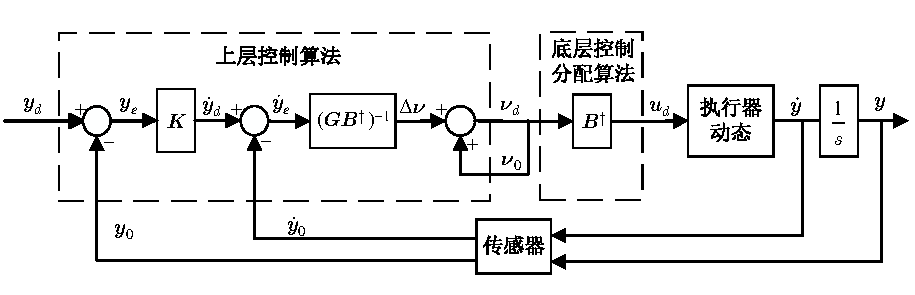
\includegraphics[scale=1]{Fig/理论框图.pdf}
		\caption{\label{理论框图}基于INDI和伪逆法的控制系统框图}
	\end{minipage}%
\end{figure}

需特别指出的是,尽管可以设计出渐进稳定的控制算法,但是受矩阵$\boldsymbol{B}$奇异特性及执行机构物理约束的影响,所推导的期望虚拟控制输入$\boldsymbol{\nu}_d$可能属于不可达集。这一现象在本质上源于伪逆法在控制分配问题中的固有局限性:当控制指令超出执行机构可达包络时,将导致控制分配问题退化为无可行解的数学约束条件,因此下文在控制分配算法的设计中将参考文献\parencite{HKXB202010026},采用优先级控制分配方法。该方法旨在通过优先级排序的方式,优先满足高优先级的控制输入分量以达到更大范围的容许控制。

\section{姿态动力学模型简化}

根据第二章的建模总结可知,DFUAV的姿态动力学模型涉及到多个系统状态变量间的耦合并且与许多模型参数和环境风速有关,尤其是角速度动态方程\eqref{eq_43}中涉及到的多源力矩模型。为便于下文姿态控制算法的设计,本节将对所总结的力矩模型进行合理且适当的简化,根据现有条件区分可控力矩与不可控力矩,然后分别处理。

根据式\ref{eq_11}可知,DFUAV在机体坐标系下的合外力矩可以分解为:
\begin{equation}
    \boldsymbol{M}^b=\boldsymbol{M}_{fan}^b+\boldsymbol{M}_{aero}^b+\boldsymbol{M}_{duct}^b+\boldsymbol{M}_{vane}^b+\boldsymbol{M}_{gyro}^b+\boldsymbol{M}_{flap}^b
    \label{3-13}
\end{equation}
由于涵道风扇的转速$\Omega$可由电调读取,机体的角速度$\boldsymbol\omega^b$可由机载的IMU测量得到,结合表\ref{DFUAV_parameters}中的模型参数,可以计算出涵道风扇的扭矩$\boldsymbol{M}_{fan}^b$和陀螺力矩$\boldsymbol{M}_{gyro}^b$。

模型假设气流相对于机体的速度在$\boldsymbol{O}_b-\boldsymbol{Z}_b$轴的分量为零,即$V_0=0$。根据式\ref{eq_20}以及式\ref{eq_22},可将涵道出口风速$V_{e}$简化为:
\begin{equation}
    V_e=\sqrt{\frac{k_{fan}}{\sigma_d\rho S}}\Omega={k_{f}}\Omega    \label{3-14}
\end{equation}
在这种假设下,涵道出口风速$V_{e}$与风扇转速$\Omega$之间呈正比关系。不妨设$V_e=k_{f}\Omega$,其中$k_{f}=\sqrt{\frac{k_{fan}}{\sigma_d\rho S}}$可以根据表\ref{DFUAV_parameters}中的参数计算得到。然后根据控制舵面的偏转角$\delta_{i}$和涵道力臂的长度,可计算出控制舵面产生的力矩$\boldsymbol{M}_{vane}^b$。

对于在固定气动面上产生的反扭距$\boldsymbol{M}_{flap}^b$,由于$V_{e}$与$\Omega$为正比关系,可将式\ref{eq_39}简化为:
\begin{equation}
    \boldsymbol{M}_{flap}^b=
    \begin{bmatrix}
    0 \\0 \\k_{flap}\Omega^2
    \end{bmatrix}
    \label{3-15}
\end{equation}

现在考虑风扇扭矩$\boldsymbol{M}_{fan}^b$、固定气动面上的反扭距$\boldsymbol{M}_{flap}^b$和控制舵面在$\boldsymbol{O}_b-\boldsymbol{Z}_b$轴的偏航力矩。根据第二章的力矩分析,仅有上述三部分分量会对机体的偏航力矩产生影响。为使机体的偏航角保持稳定,有如下关系:
\begin{equation}
    \begin{gathered}
    -k_q\Omega^2+k_{flap}\Omega^2+k_{\delta}k_f^2 l_2(\delta_1 + \delta_2 + \delta_3 + \delta_4)\Omega^2=0
     \\
     \Rightarrow
    -k_q+k_{flap}+k_{\delta}k_f^2 l_2(\delta_1 + \delta_2 + \delta_3 + \delta_4)=0
    \end{gathered}
    \label{3-16}
\end{equation}
式\ref{3-15}中等式约去风扇转速变量$\Omega$后,只有控制舵面的偏转角是变量,其他均为确定的模型参数。这表明了当机体偏航角稳定时,所需的控制舵面偏转角是一定的。由于$k_{flap}$与固定气动面的设计形状有关,不失一般性,本文假设固定气动面在恰当的设计下可以使得$k_{flap}=k_{q}$,即:
\begin{equation}
    \boldsymbol{M}_{flap}^b + \boldsymbol{M}_{fan}^b = \boldsymbol{0}
\label{3-17}
\end{equation}

对于在机身上产生的气动力矩$\boldsymbol{M}_{aero}^b$和由于涵道翼型产生的力矩$\boldsymbol{M}_{duct}^b$,由于机体相对于气流的速度$\boldsymbol{V}_a^b$在现有条件下是未知的,所以将其视为不可控力矩来作为未建模动态力矩。使用$\boldsymbol{M}_{a}^b$统一表示:
\begin{equation}
    \boldsymbol{M}_{a}^b=\boldsymbol{M}_{aero}^b+\boldsymbol{M}_{duct}^b
    \label{3-18}
\end{equation}

$\boldsymbol{M}_{a}^b$可以描述为地面坐标系下的速度$\boldsymbol{V}^e$、姿态$\boldsymbol{\eta}$和环境风速$\boldsymbol{W}^e$的函数,即:
\begin{equation}
    \boldsymbol{M}_{a}^b=\boldsymbol{M}_{a}^b(\boldsymbol{V}^e,\boldsymbol{\eta},\boldsymbol{W}^e)
    \label{3-19}
\end{equation}

综合以上分析,简化后的气动力矩模型可以写为:
\begin{equation}
    \boldsymbol{M}^b=\boldsymbol{M}_{vane}^b+\boldsymbol{M}_{gyro}^b+\boldsymbol{M}_{a}^b
    \label{3-20}
\end{equation}
与力矩模型相关的角速度动态方程对应的可以简写为:
\begin{equation}
    \begin{aligned}
        \dot{p}  &=\frac{1}{J_x}\Bigg\{ (J_y-J_z)qr+
        \big[- l_1k_\delta V_e^2(\delta_1 - \delta_3)-J_{fan}\Omega{q} +\boldsymbol{M}_{ax}^b\big]\Bigg\} \\
        \dot{q}  &=\frac{1}{J_y}\Bigg\{ (J_z-J_x)pr+
        \big[l_1k_\delta V_e^2(\delta_4 - \delta_2)+J_{fan}\Omega{p} +\boldsymbol{M}_{ay}^b\big]\Bigg\} \\
        \dot{r}  &=\frac{1}{J_z}\Bigg\{ (J_x-J_y)pq+
        \left[l_2k_\delta V_e^2(\delta_1 + \delta_2 + \delta_3 + \delta_4) + \boldsymbol{M}_{az}^b\right]
        \Bigg\}
    \end{aligned}
    \label{3-21}
\end{equation}
上述简化的力矩模型将可控力矩与不可控力矩分开。控制舵面合力矩$\boldsymbol{M}_{vane}^b$作为可控力矩由下文设计的姿态控制算法来计算期望力矩(即期望的控制舵面偏转角度)。陀螺力矩$\boldsymbol{M}_{gyro}^b$同样作为可控力矩,但该力矩会对DFUAV的姿态造成负面影响,下文将根据其产生的机理设计对应的陀螺力矩补偿算法加以补偿。而$\boldsymbol{M}_{a}^b$作为不可控力矩将通过姿态控制算法在在线补偿。

\section{基于INDI和优先级控制分配的姿态控制方案}

根据本章开篇时的分析,姿态控制算法设计的核心在于如何对难以测得的力矩进行在线补偿。在第二节姿态动力学模型简化中,将难以测得的力矩视为了未建模动态力矩$\boldsymbol{M}_{a}^b$。基于INDI的控制架构设计,其优势主要体现在模型的鲁棒性与未建模误差的动态补偿能力。式\eqref{3-21}中的形式已十分适用于INDI姿态控制器的设计:一方面,姿态子系统的输入通道的模型机理已经明确,由四片独立的控制舵面产生偏转角作为输入信号;另一方面,由于未建模动态力矩$\boldsymbol{M}_{a}^b$作用于角加速度,所以可用机载IMU高频测量角速度并估算角加速度,并根据INDI的增量式求逆策略在线补偿未建模动态力矩$\boldsymbol{M}_{a}^b$。在所构建的控制架构中,控制输入分为两部分:INDI输入与反馈输入。INDI输入针对$\boldsymbol{M}_{a}^b$进行补偿,将非线性系统转化为线性形式;而反馈输入针对此线性形式设计反馈控制律,保证系统的稳定性和鲁棒性。

根据优先级控制分配的思想,需要将控制输入分量进行优先级排序。由于INDI输入包含对未建模动态力矩的补偿,反馈输入使用线性的状态反馈设计,与系统响应相关。系统能够稳定运行的前提是首先消除未建模动态力矩的影响,将非线性系统化为线性系统,然后再设计反馈控制律,确保系统的稳定性与响应能力。因此本文中将INDI输入视为高优先级分量,反馈输入视为低优先级分量。确保INDI输入不会产生分配误差,在控制舵面受到物理约束的情况下仅在反馈输入中产生分配误差。具体而言,这种划分方法可以在一定程度上避免系统输出耦合现象\cite{HKXB202010026}。

\subsection{INDI姿态控制架构}

对于大部分无人机姿态运动控制,常采用基于欧拉角参数化的局部线性化方法,滚转角、俯仰角和偏航角三个通道分别作为控制目标单独控制,使得无人机的旋转过程被线性化处理。但是不同于位置动态方程\eqref{eq_40},欧拉角动态方程\eqref{eq_42}将三个姿态通道耦合在一起。实际上,无人机的姿态属于$SO(3)$上的流形结构,任何姿态变化都被视为流形上的测地线运动。而传统的局部线性化跟踪姿态的方法相当于在流形的切空间进行局部线性逼近,这种线性化处理方式导致了姿态轨迹生成过程中的不连续性,丢失了流形的曲率信息,所以在机动飞行时会导致姿态跟踪误差变大。因此本文参考文献\parencite{10.1115/1.4052714}在$SO(3)$上考虑姿态误差的表示。

由于旋转矩阵$\boldsymbol{R}\in{SO(3)}$,姿态欧拉角$\boldsymbol{\eta}\in\mathbb{R}^3$,因此定义符号$[.]_\times$表示映射关系$\mathbb{R}^3\to SO(3)$,$(.)^\vee$表示对应的逆映射$SO(3)\to\mathbb{R}^3$。对于任意姿态$\boldsymbol{\eta}=[\varphi \quad \theta \quad \psi]^T$,对应的矩阵形式可以表示为:
\begin{equation}
    \boldsymbol{R}=[\boldsymbol{\eta}]_\times=
    \begin{bmatrix}
    0 & -\psi & \theta \\
    \psi & 0 & -\varphi \\
    -\theta & \varphi & 0
    \end{bmatrix}
    \label{3-22}
\end{equation}

假设期望姿态为$\boldsymbol{\eta}_d$,当前姿态为$\boldsymbol{\eta}$,对应的矩阵形式分别为$\boldsymbol{R}_d$和$\boldsymbol{R}$。则在${SO(3)}$上的姿态误差可以表示为:
\begin{equation}
    \boldsymbol{e}_R=\dfrac{1}{2}(\boldsymbol{R}_d^T\boldsymbol{R}-\boldsymbol{R}^T\boldsymbol{R}_d)^\vee\in \mathbb{R}^3
    \label{3-23}
\end{equation}

因此期望的姿态欧拉角变化率可以表示为:
\begin{equation}
    \dot{\boldsymbol{\eta}}_1=-\boldsymbol{K}_R\boldsymbol{e}_R
    \label{3-24}
\end{equation}
其中$\boldsymbol{K}_R=diag({K}_{R\varphi},{K}_{R\theta},{K}_{R\psi})$为姿态误差的正定增益矩阵。式\eqref{3-24}所示的作差方式类似于于反馈信号减去给定信号,所以需要加负号。

为提高系统的响应速度,确保快速跟踪期望姿态,引入微分前馈策略:
\begin{equation}
    \dot{\boldsymbol{\eta}}_2=\frac{d\boldsymbol{\eta}_d}{dt}
    \label{3-25}
\end{equation}

结合式\eqref{eq_10}、式\eqref{3-24}和式\eqref{3-25},期望的机体角速度$\boldsymbol\omega^{b}_d$可以表示为:
\begin{equation}
    \boldsymbol{\omega}^{b}_d=\boldsymbol{Q}^{-1}( \dot{\boldsymbol{\eta}}_1+ \dot{\boldsymbol{\eta}}_2)
    \label{3-26}
\end{equation}

接下来考虑与动力学相关的角速度动态,包含了可控力矩与不可控力矩。如前文所述,DFUAV姿态子系统的控制输入为四片相互独立的控制舵面的偏转角$\delta_i$,由四个偏转角度的组合产生用于控制机体姿态的俯仰力矩、滚转力矩和偏航力矩,因此姿态子系统中存在执行机构的冗余,存在过驱动的问题。引入虚拟控制输入$\boldsymbol{\nu}\in\mathbb{R}^3$将姿态控制算法与控制分配算法分开:
\begin{equation}
    \boldsymbol{\nu}=
    \begin{bmatrix}
    {\nu}_x \\ {\nu}_y \\ {\nu}_z
    \end{bmatrix}=\boldsymbol{B}
    \begin{bmatrix}
    \delta_1 \\ \delta_2 \\ \delta_3 \\ \delta_4
    \end{bmatrix}
    \label{3-27}
\end{equation}
其中矩阵$\boldsymbol{B}$表示四片独立控制舵面偏转角到三维虚拟控制输入的映射矩阵,有$\boldsymbol{B}\in\mathbb{R}^{3\times4}$。

结合式\eqref{eq_10}、式\eqref{eq_36}、式\eqref{3-14}和式\eqref{3-27},可以将可控的控制舵面力矩重写为模块化形式:
\begin{equation}
    (\boldsymbol{J}^b)^{-1}\boldsymbol{M}_{vane}^b=\boldsymbol{H}_{vane}\boldsymbol{\nu}\Omega^2
    \label{3-28}
\end{equation}
其中
\begin{gather}
\left.\boldsymbol{H}_{vane}\triangleq k_{\delta}k_f^2\left[
    \begin{array}
    {ccc}2J_x^{-1}l_1 & & \\
        & 2J_y^{-1}l_1 & \\
        & & 4J_z^{-1}l_2
    \end{array}\right.\right]\in\mathbb{R}^{3\times3}
    \label{3-29}\\
    \boldsymbol{B}=
    \begin{bmatrix}
    -0.5 & 0 & 0.5 & 0 \\
    0 & -0.5 & 0 & 0.5 \\
    0.25 & 0.25 & 0.25 & 0.25
    \end{bmatrix}
    \label{3-30}
\end{gather}
经过式\eqref{3-28}的模块化处理,由原本的从控制舵面角度到控制力矩的映射转变为了从控制舵面角度到虚拟控制输入的映射。在此过程中,映射矩阵剔除了所有与模型相关参数项。

对于可控的陀螺力矩$\boldsymbol{M}_{gyro}^b$,根据式\eqref{eq_10}和式\ref{eq_38},可将其模块化表示为:
\begin{equation}
    (\boldsymbol{J}^b)^{-1}\boldsymbol{M}_{gyro}^b=\boldsymbol{H}_{gyro}(\boldsymbol{\omega}^b)\Omega
    \label{3-31}
\end{equation}
其中
\begin{equation}
    \boldsymbol{H}_{gyro}(\boldsymbol{\omega}^b) \triangleq J_{fan}[-J_x^{-1}q\quad J_y^{-1}p\quad0]^T\in\mathbb{R}^{3}
    \label{3-32}
\end{equation}

对于不可控的气动力矩$\boldsymbol{M}_{a}^b$,将其与式\eqref{eq_10}中的非线性项$(\boldsymbol{J}^b\boldsymbol{\omega}^b\times\boldsymbol{\omega}^b)$一同处理,表示为与地面坐标系下的速度$\boldsymbol{V}^e$、姿态$\boldsymbol{\eta}$、环境风速$\boldsymbol{W}^e$和机体角速度$\boldsymbol{\omega}^b$有关的函数:
\begin{equation}
    ({\boldsymbol{J}^b})^{-1}(\boldsymbol{M}_{a}^b+\boldsymbol{J}\boldsymbol{\omega}^b\times\boldsymbol{\omega}^b)\triangleq \boldsymbol{L}(\boldsymbol{V}^e,\boldsymbol{\eta},\boldsymbol{W}^e,\boldsymbol{\omega}^b)\in\mathbb{R}^3
    \label{3-33}
\end{equation}

结合式\eqref{3-28}、式\eqref{3-31}和式\eqref{3-33},角速度动态方程可以被模块化表示为:
\begin{equation}
    \boldsymbol{\dot{\omega}}^b=\boldsymbol{H}_{vane}\boldsymbol{\nu}\Omega^2+\boldsymbol{H}_{gyro}(\boldsymbol{\omega}^b)\Omega+\boldsymbol{L}(\boldsymbol{V}^e,\boldsymbol{\eta},\boldsymbol{W}^e,\boldsymbol{\omega}^b)
    \label{3-34}
\end{equation}
可以直接在该模型的基础上应用INDI,而无需考虑控制分配问题。根据本章第一节介绍的INDI理论,为了得到$\boldsymbol{\dot{\omega}}^b$的增量表达式,对公式\eqref{3-34}在其工作点处(使用下标$(.)_0$表示)作一阶泰勒展开:
\begin{equation}
    \begin{aligned}
    \boldsymbol{\dot{\omega}}^b&=\boldsymbol{H}_{vane}\boldsymbol{\nu}\Omega^2+\boldsymbol{H}_{gyro}(\boldsymbol{\omega}^b)\Omega+\boldsymbol{L}(\boldsymbol{V}^e,\boldsymbol{\eta},\boldsymbol{W}^e,\boldsymbol{\omega}^b)\\
    &=\boldsymbol{H}_{vane}\boldsymbol{\nu}_0\Omega_0^2+\boldsymbol{H}_{gyro}(\boldsymbol{\omega}_0^b)\Omega_0+\boldsymbol{L}_0\\
    & +\left.\frac{\partial(\boldsymbol{H}_{vane}\boldsymbol{\nu}\Omega^2)}{\partial\boldsymbol{\nu}}\right|_{\boldsymbol{\nu}=\boldsymbol{\nu}_0}(\boldsymbol{\nu}-\boldsymbol{\nu}_0)
    +\left.\bigg[\frac{\partial(\boldsymbol{H}_{vane}\boldsymbol{\nu}\Omega^2)}{\partial\Omega}+\frac{\partial(\boldsymbol{H}_{gyro}\Omega)}{\partial\Omega}\bigg]\right|_{\Omega=\Omega_0}
    (\Omega-\Omega_0) \\
     & +\left.\bigg[\frac{\partial(\boldsymbol{H}_{gyro}\Omega)}{\partial\boldsymbol{\omega}^{b}}+\frac{\partial\boldsymbol{L}}{\partial\boldsymbol{\omega}^{b}}\bigg]\right|_{\boldsymbol{\omega}^{b}=\boldsymbol{\omega}_{0}^{b}}(\boldsymbol{\omega}^{b}-\boldsymbol{\omega}_{0}^{b})\\
    & +\left.\frac{\partial\boldsymbol{L}}{\partial\boldsymbol{V}^{e}}\right|_{\boldsymbol{V}^{e}=\boldsymbol{V}_{0}^{e}}
    (\boldsymbol{V}^{e}-\boldsymbol{V}_{0}^{e})
    +\left.\frac{\partial\boldsymbol{L}}{\partial\boldsymbol{\eta}}\right|_{\boldsymbol{\eta}=\boldsymbol{\eta}_{0}}(\boldsymbol{\eta}-\boldsymbol{\eta}_{0})
    +\left. \frac{\partial\boldsymbol{L}}{\partial\boldsymbol{W}^e}\right|_{\boldsymbol{W}^e=\boldsymbol{W}_0{}^e}(\boldsymbol{W}^e-\boldsymbol{W}_0{}^e)
    \end{aligned}
    \label{3-35}
\end{equation}
展开式中的第一项$\boldsymbol{H}_{vane}\boldsymbol{\nu}_0\Omega_0^2+\boldsymbol{H}_{gyro}(\boldsymbol{\omega}_0^b)\Omega_0+\boldsymbol{L}_0$等价于工作点处的角加速度,可以由机载IMU测量的角速度经过差分滤波得到:
\begin{equation}
    \boldsymbol{\dot{\omega}}^b_0=\boldsymbol{H}_{vane}\boldsymbol{\nu}_0\Omega_0^2+\boldsymbol{H}_{gyro}(\boldsymbol{\omega}_0^b)\Omega_0+\boldsymbol{L}_0
    \label{3-36}
\end{equation}

展开式中的其他项是关于系统内部状态变量$(\boldsymbol{V}^e,\boldsymbol{\eta},\boldsymbol{\omega}^b)$、系统控制输入$(\boldsymbol{\nu},\Omega)$和外部扰动$\boldsymbol{W^e}$的一阶偏导数项。根据本章第一小节介绍的时间尺度分离法则,认为在角加速度的输入信号的时间尺度内,系统内部状态变量包括速度、姿态和机体角速度的变化是缓慢的,因此可以将这些状态变量的一阶偏导数项视为0:
\begin{equation}
    \begin{cases}
        \boldsymbol{V}^e-\boldsymbol{V}_0^e\approx0 \\
        \boldsymbol{\eta}-\boldsymbol{\eta}_0\approx0 \\
        \boldsymbol{\omega}^b-\boldsymbol{\omega}_0^b\approx0
    \end{cases}
    \label{3-37}
\end{equation}

在无人机控制中,执行机构(如电机、舵机等)可在数十毫秒的时间尺度内完成控制指令的执行,产生所需的力与力矩。而机体的速度、姿态等状态变量受空气动力阻尼、质量惯性等因素的制约,其动态过程一般落后于执行机构响应1-2个数量级,因此上述假设是合理的。此外,对于外部环境风速扰动$\boldsymbol{W}^e$的变化是未知并且难以预测的,因此假定$(\boldsymbol{W}^e-\boldsymbol{W}_0^e\approx0)$。但此假设并没有排除外部环境风速扰动对系统的影响,缓慢变化的自然风对姿态造成的影响已被考虑在$\boldsymbol{L}_0$中。而应对快速变化的风速扰动则取决于所设计的姿态控制器的鲁棒性。

其余关于系统控制输入的偏导数项如下:
\begin{equation}
    \begin{gathered}
    \left.\frac{\partial(\boldsymbol{H}_{vane}\boldsymbol{\nu}\Omega^2)}{\partial\boldsymbol{\nu}}\right|_{\boldsymbol{\nu}=\boldsymbol{\nu}_0}(\boldsymbol{\nu}-\boldsymbol{\nu}_0)=\boldsymbol{H}_{vane}\Omega_0^2(\boldsymbol{\nu}-\boldsymbol{\nu}_0) \\
    \left.\bigg[\frac{\partial(\boldsymbol{H}_{vane}\boldsymbol{\nu}\Omega^2)}{\partial\Omega}+\frac{\partial(\boldsymbol{H}_{gyro}\Omega)}{\partial\Omega}\bigg]\right|_{\Omega=\Omega_0}(\Omega-\Omega_0)=\big[2\boldsymbol{H}_{vane}\boldsymbol{\nu}_0\Omega_0+\boldsymbol{H}_{gyro}(\boldsymbol{\omega}_0^b)\big](\Omega-\Omega_0)
    \end{gathered}
    \label{3-38}
\end{equation}

因此,角速度动态的一阶泰勒展开式\eqref{3-35}近似可以表示为:
\begin{equation}
    \boldsymbol{\dot{\omega}}^b=\boldsymbol{\dot{\omega}}_0^b+\boldsymbol{H}_{vane}\Omega_0^2(\boldsymbol{\nu}-\boldsymbol{\nu}_0)+\big[2\boldsymbol{H}_{vane}\boldsymbol{\nu}_0\Omega_0+\boldsymbol{H}_{gyro}(\boldsymbol{\omega}_0^b)\big](\Omega-\Omega_0)
    \label{3-39}
\end{equation}

值得一提的是,风扇转速$\Omega$作为速度控制的输入信号并不直接参与姿态控制。简化后的角速度动态(即式\eqref{3-21})中与$\Omega$相关的项均与陀螺力矩$\boldsymbol{M}_{gyro}^b$有关,将由下文设计的陀螺力矩补偿算法补偿。因此$\Omega$不被视为姿态控制中输入信号的一部分,可以将$\Omega$作为在角速度动态中的已知参数,该参数可以从速度环设计中得到。为了简便表示,采用以下记号:
\begin{equation}
    \boldsymbol{T}(\Omega)=\big[2\boldsymbol{H}_{vane}\boldsymbol{\nu}_0\Omega_0+\boldsymbol{H}_{gyro}(\boldsymbol{\omega}_0^b)\big](\Omega-\Omega_0)\in\mathbb{R}^3
    \label{3-40}
\end{equation}

将式\eqref{3-40}代入式\eqref{3-39},可以得到角速度$\boldsymbol{\omega}^b$动态的增量表达式:
\begin{equation}
    \begin{aligned}
    \boldsymbol{\dot{\omega}}^b&=\boldsymbol{\dot{\omega}}_0^b+\boldsymbol{H}_{vane}\Omega_0^2(\boldsymbol{\nu}-\boldsymbol{\nu}_0)+\boldsymbol{T}(\Omega)\\
    &=\begin{bmatrix}\dot{p}_0 \\ \dot{q}_0 \\ \dot{r}_0 \end{bmatrix}
    + k_{\delta}k_f^2\Omega_0^2
    \left[\begin{array}{ccc}2J_x^{-1}l_1 & & \\& 2J_y^{-1}l_1 & \\& & 4J_z^{-1}l_2\end{array}\right]
    \left(\begin{bmatrix}\nu_{x} \\ \nu_{y} \\ \nu_{z}\end{bmatrix}
    -\begin{bmatrix}\nu_{x0} \\ \nu_{y0} \\ \nu_{z0}\end{bmatrix}\right)
    +  \begin{bmatrix}T_{x}(\Omega) \\ T_{y}(\Omega) \\ T_{z}(\Omega)
    \end{bmatrix}
    \end{aligned}
    \label{3-41}
\end{equation}

INDI通过对式\eqref{3-41}进行求逆,来得到期望的虚拟控制输入的增量表达式:
\begin{equation}
    \begin{aligned}
        \boldsymbol{\nu}_d&=(\boldsymbol{H}_{vane}\Omega_0^2)^{-1}\Big\{\boldsymbol{\mu} -\big[\boldsymbol{\dot{\omega}}_0^b+\boldsymbol{T}(\Omega)\big]\Big\}+\boldsymbol{\nu}_0\\
        &=\frac{1}{k_{\delta}k_f^2\Omega_0^2}
        \left[\begin{array}{ccc}2J_x^{-1}l_1 & & \\& 2J_y^{-1}l_1 & \\& & 4J_z^{-1}l_2\end{array}\right]^{-1}
        \left\{\begin{bmatrix}\mu_{x} \\ \mu_{y} \\ \mu_{z}\end{bmatrix}
        -\left (\begin{bmatrix}\dot{p}_0 \\ \dot{q}_0 \\ \dot{r}_0 \end{bmatrix}+\begin{bmatrix}T_{x}(\Omega) \\ T_{y}(\Omega) \\ T_{z}(\Omega)
        \end{bmatrix}\right )\right\}
        +  \begin{bmatrix}\nu_{x0} \\ \nu_{y0} \\ \nu_{z0}\end{bmatrix}
    \end{aligned}
    \label{3-42}
\end{equation}

其中,虚拟输入项$\boldsymbol{\nu}$被$\boldsymbol{\nu}_d$替换,表明是期望的输入。类似地,$\boldsymbol{\Omega}$被替换为$\boldsymbol{\Omega}_d$。

将式\eqref{3-42}代入式\eqref{3-41},得到线性化的角速度动态方程:
\begin{equation}
    \dot{\boldsymbol \omega}^b=\boldsymbol{\mu}
    \label{3-43}
\end{equation}

最终,通过以下比例反馈律,可以得到稳定的角速度子系统:
\begin{equation}
    \boldsymbol{\mu}=\boldsymbol{K}_{\omega}(\boldsymbol{\omega}_d^b-\boldsymbol{\omega}^b)
    \label{3-44}
\end{equation}

将式\eqref{3-44}代入式\eqref{3-43}中可以得到:
\begin{equation}
    \dot{\boldsymbol \omega}^b=\boldsymbol{K}_{\omega}(\boldsymbol{\omega}_d^b-\boldsymbol{\omega}^b)
    \label{3-45}
\end{equation}
其中$\boldsymbol{K}_\omega=diag({K}_{\omega p},{K}_{\omega q},{K}_{\omega r})$为正反馈增益矩阵。

基于INDI的控制思想已经把非线性角速度动力学方程\eqref{3-34}简化为了一个一阶积分系统\eqref{3-43},因此采用单一的比例控制器就可以确保闭环系统的稳定性,只需要保证反馈增益为正,而不管其具体取值。这进一步提供了一个指导,可以分别确定闭环系统的静态平衡点和动态性能。因此结合式\eqref{3-44},可以将式\eqref{3-42}可以分为两部分:
\begin{equation}
    \boldsymbol{\nu}_d=\boldsymbol{\nu}_i + \boldsymbol{\nu}_f
    \label{3-46}
\end{equation}
其中$\boldsymbol{\nu}_i$定义为INDI输入,$\boldsymbol{\nu}_f$定义为反馈输入,具体形式为:
\begin{equation}
    \begin{aligned}
        \boldsymbol{\nu}_i&=-(\boldsymbol{H}_{vane}\Omega_0^2)^{-1} \big[\boldsymbol{\dot{\omega}}_0^b+\boldsymbol{T}_d(\Omega)\big]+\boldsymbol{\nu}_0\\
        &=-\frac{1}{k_{\delta}k_f^2\Omega_0^2}
        \left[\begin{array}{ccc}2J_x^{-1}l_1 & & \\& 2J_y^{-1}l_1 & \\& & 4J_z^{-1}l_2\end{array}\right]^{-1}
        \left (\begin{bmatrix}\dot{p}_0 \\ \dot{q}_0 \\ \dot{r}_0 \end{bmatrix}+\begin{bmatrix}T_{x}(\Omega) \\ T_{y}(\Omega) \\ T_{z}(\Omega)
        \end{bmatrix}\right )
        +  \begin{bmatrix}\nu_{x0} \\ \nu_{y0} \\ \nu_{z0}\end{bmatrix}
    \end{aligned}
    \label{3-47}
\end{equation}
\begin{equation}
    \begin{aligned}
        \boldsymbol{\nu}_f&=(\boldsymbol{H}_{vane}\Omega_0^2)^{-1}\boldsymbol{K}_{\omega}(\boldsymbol{\omega}_d^b-\boldsymbol{\omega}^b)\\
        &=\frac{1}{k_{\delta}k_f^2\Omega_0^2}
        \left[\begin{array}{ccc}2J_x^{-1}l_1 & & \\& 2J_y^{-1}l_1 & \\& & 4J_z^{-1}l_2\end{array}\right]^{-1}
        \left[\begin{array}{ccc}{K}_{\omega 1} & & \\& {K}_{\omega 2} & \\& & {K}_{\omega 3}\end{array}\right]
        \left (\begin{bmatrix}\dot{p}_d \\ \dot{q}_d \\ \dot{r}_d \end{bmatrix}-\begin{bmatrix}\dot{p} \\ \dot{q} \\ \dot{r}
        \end{bmatrix}\right )
    \end{aligned}
    \label{3-48}
\end{equation}

INDI采用增量控制策略,将未建模动态力矩项$\boldsymbol{M}_{a}^b$和角速度动力学耦合项$\boldsymbol{J}\boldsymbol{\omega}^b\times\boldsymbol{\omega}^b$造成的影响放在了$\dot {\boldsymbol{\omega}}_0^b$中处理。在每一个工作点计算的INDI输入都是基于上一个工作点的INDI输入加上模型误差、阵风扰动以及风扇转速输入对相邻两个工作点之间的角加速度影响。因此,模型误差不会随着时间进行累计,而是在每一个工作点实时补偿。而系统的稳定性由基于误差的角速度反馈来保证。

根据上述分析,INDI输入的计算依赖于机体的角加速度值$\dot {\boldsymbol{\omega}}_0^b$,在现有条件下,该值可以通过对机体陀螺仪测量的相邻两个采样点的角速度进行一阶差分得到:
\begin{equation}
    \dot{\boldsymbol{\omega}}^b(k)=\frac{
        \begin{bmatrix}
        \boldsymbol{\omega}^b(k)-\boldsymbol{\omega}^b(k-1)
        \end{bmatrix}}{\Delta t}
    \label{3-49}
\end{equation}
其中$\Delta t$是陀螺仪传感器的采样时间,$k$为传感器的采样点,泰勒展开式中的工作点一般选取为当前的采样时刻。因此INDI也被称为基于传感器的方法。

在飞行控制系统的工程实现中,为了提高姿态控制器的响应速度和控制精度,$\Delta t$应该在条件允许的情况下尽可能小。但是传感器测量得到的角速度原始值会受到机体震动和外部扰动等因素的影响,难免会有噪声,对原始值进行差分运算后会放大这种噪声的影响,采样时间越小,噪声影响越大。因此在实际应用中,需要对角速度进行滤波处理。但是滤波处理就会在角加速度的计算中引入延迟,由于INDI是将角速度动力学方程在工作点处进行一阶泰勒展开,所以需要保证展开式\eqref{3-41}中所有下标为0的项都位于同一工作点。一种方法是对角加速度进行预测,如采用卡尔曼滤波器对其进行预测来补偿相位滞后,但是这种方法需要对角加速度进行额外的建模,并且角速度收到的的干扰也无法预测。或者采用多个加速度计数据融合来直接测量角加速度,但是这种方式会导致机载航电系统设计过于复杂,并且加速度计受机体震动影响也较大,多传感器数据融合的精度难以有效保证。

因此,本文针对所有下标为0的项进行同步滤波处理,除了角加速度项外,还包括虚拟控制输入项和风扇转速输入项。文献\parencite{smeurAdaptiveIncrementalNonlinear2015,smeurCascadedIncrementalNonlinear2018b}通过四旋翼飞行实验表明这种处理方式的可行性。考虑到陀螺仪传感器的高频噪声影响,本文实验使用的滤波器是二阶巴特沃斯(Butterworth)低通滤波器,滤波器截止频率的具体数值应该根据飞行过程中信号的频率成分、带宽和噪声水平来综合确定。对于本文使用的DFUAV,滤波器截止频率为30Hz。为加以区分,所有下标为0的项经过滤波器滤波后,使用下标$(.)_s$表示。

\subsection{陀螺力矩补偿}

在基于INDI的控制架构中,陀螺力矩$\boldsymbol{M}_{gyro}^b$分量蕴含在了$\boldsymbol{T}(\Omega)$中(见式\eqref{3-40}),该力矩的存在会在姿态发生改变时影响姿态跟踪精度。因此,为了消除陀螺力矩对姿态控制的影响,需要在INDI输入$\boldsymbol{\nu}_i$中(见式\eqref{3-47})对其进行补偿。由于姿态子系统的控制输入为控制舵面的偏转角度,并且根据式\eqref{eq_38}可知陀螺力矩的机理已十分明确。所以可以将陀螺力矩对应的值等价转化为虚拟控制输入量,然后在$\boldsymbol{\nu}_i$中减去该分量,即可对陀螺力矩造成的负面影响进行补偿。

根据式\eqref{eq_35}、\eqref{eq_36}和式\eqref{3-14},在现有条件下可用于计算的控制舵面力矩可表示为:
\begin{gather}
    \boldsymbol{M}_{vane}^b=k_{\delta}k_f^2\Omega^2\begin{bmatrix}
        -l_1 & 0 & l_1 & 0 \\
        0 & -l_1 & 0 & l_1 \\
        l_2 & l_2 & l_2 & l_2
        \end{bmatrix}\boldsymbol{{\delta}}
    \label{3-50}
\end{gather}

将式\eqref{3-27}代入式\eqref{3-50}可得:
\begin{gather}
    \boldsymbol{M}_{vane}^b=k_{\delta}k_f^2\Omega^2\begin{bmatrix}
        -l_1 & 0 & l_1 & 0 \\
        0 & -l_1 & 0 & l_1 \\
        l_2 & l_2 & l_2 & l_2
        \end{bmatrix}\boldsymbol{B}^{\dagger}\boldsymbol{\nu}
    \label{3-51}
\end{gather}
根据式\eqref{3-12}以及式\eqref{3-30}中矩阵B的值,可以计算得到$\boldsymbol{B}^{\dagger}$为:
\begin{gather}
    \boldsymbol{B}^{\dagger}=
        \begin{bmatrix}
        -1 & 0 & 1 \\
        0 & -1 & 1  \\
        1 & 0 & 1 \\
        0 & 1 & 1
        \end{bmatrix}
    \label{3-52}
\end{gather}

如果直接计算与陀螺力矩等效的控制舵面的偏转角度,那么就有可能在在实际控制中出现控制舵面的偏转角度超过其可行范围的情况。这是因为与陀螺力矩等效的控制舵面的偏转角度未经过控制分配算法的优化分配,导致期望的控制效果与实际不符。因此,此处计算与陀螺力矩等效的虚拟控制输入以便于INDI输入$\boldsymbol{\nu}_i$一起参与优先级控制分配。

令式\eqref{eq_38}所描述的陀螺力矩和式\eqref{3-51}描述的控制舵面力矩相等,可以得到与陀螺力矩等效的虚拟控制输入$\boldsymbol{\nu}_{gyro}$:
\begin{equation}
    \begin{gathered}
        \boldsymbol{M}_{gyro}^b=\boldsymbol{M}_{vane}^b\\
        \Rightarrow J_{fan}\Omega\begin{bmatrix}-q \\ p \\ 0\end{bmatrix}
        =
        k_{\delta}k_f^2\Omega^2\begin{bmatrix}
            -l_1 & 0 & l_1 & 0 \\
            0 & -l_1 & 0 & l_1 \\
            l_2 & l_2 & l_2 & l_2
            \end{bmatrix}\boldsymbol{B}^{\dagger}\boldsymbol{\nu}_{gyro}\\
        \Rightarrow \boldsymbol{\nu}_{gyro}=\frac{J_{fan}}{k_{\delta}k_f^2\Omega}\boldsymbol{B}\begin{bmatrix}
            -l_1 & 0 & l_1 & 0 \\
            0 & -l_1 & 0 & l_1 \\
            l_2 & l_2 & l_2 & l_2
            \end{bmatrix}^{\dagger}\begin{bmatrix}-q \\ p \\ 0\end{bmatrix}
        \label{3-53}
    \end{gathered}
\end{equation}

因此,加入陀螺力矩补偿后的INDI输入$\boldsymbol{\nu}_i$为:
\begin{equation}
    \begin{aligned}
        \boldsymbol{\nu}_i&=-(\boldsymbol{H}_{vane}\Omega_0^2)^{-1} \big[\boldsymbol{\dot{\omega}}_0^b+\boldsymbol{T}_d(\Omega)\big]+\boldsymbol{\nu}_0-\boldsymbol{\nu}_{gyro}
    \end{aligned}
    \label{3-54}
\end{equation}
其中$\boldsymbol{\nu}_{gyro}$表达式中的风扇转速项$\Omega$和角速度项$\boldsymbol{\omega}^b$都需要同步滤波。

\subsection{优先级控制分配}

由于DFUAV的特殊构型,飞行过程中由期望控制输入计算出的控制舵面偏转角很可能超出其物理约束,所以底层设计用于解决控制分配问题。该问题可以描述为对于给定的三维期望虚拟控制输入$\boldsymbol{\nu}_d$,找到一组四片控制舵面的偏转角度在容许控制集合的范围内$\boldsymbol{\delta}_d\in \boldsymbol{U}$使得$\boldsymbol{\nu}_d=\boldsymbol{B}\boldsymbol{\delta}_d$,或者在无法找到这样一组解的情况下,需要找到一组最优解使得分配误差$\boldsymbol{\nu}_d-\boldsymbol{B}\boldsymbol{\delta}_d$最小化。容许控制集合$\boldsymbol{U}$由下式定义:
\begin{equation}
    \boldsymbol{U}=\{\boldsymbol{\delta}\in\mathbb{R}^4|-\delta_m\leq\delta_i\leq\delta_m,i=1,2,3,4\}
    \label{3-55}
\end{equation}

对应的,虚拟控制输入$\boldsymbol{\nu}$的可达集合$\boldsymbol\Phi$表示为:
\begin{equation}
    \boldsymbol\Phi=\left\{\boldsymbol{\nu}\in\mathbb{R}^3|\boldsymbol{\nu}=\boldsymbol{B}\boldsymbol{\delta},\boldsymbol{\delta}\in \boldsymbol{U}\right\}
    \label{3-56}
\end{equation}
其中$\boldsymbol{B}$由式\eqref{3-30}给出。

为了实现控制分配的目标,广泛采用的方法是直接计算矩阵$\boldsymbol{B}$的伪逆矩阵$\boldsymbol{B}^{\dagger}$,然后计算$\boldsymbol{\delta}_d$:
\begin{equation}
    \boldsymbol{\delta}_d=\boldsymbol{B}^{\dagger}\boldsymbol{\nu}_d
    \label{3-57}
\end{equation}

使用伪逆方法的优点是计算简单,易于理解。但是在工作点的约束边界区,即使$\boldsymbol{\nu}_d$保持在可达集合内,伪逆法计算出的$\boldsymbol{\delta}_d$中的部分分量也可能会超出约束边界,即$\boldsymbol{\delta}\notin\boldsymbol{U}$。在这种情况下,伪逆法会计算出一个基于某种性能指标的次最优解,次最优解可能有多种选择,所以次最优解之间亦有优劣之分。伪逆法没有对这些解进行优先级排序,因此无法保证次最优解的唯一性。

为了弥补伪逆方法的不足,采用优先级控制分配方法,将期望的虚拟控制输入进行矢量分解划分各自的优先级,优先满足高优先级的控制输入分量。式\eqref{3-46}已将期望的虚拟控制输入$\boldsymbol{\nu}_d$分为两部分,即$\boldsymbol{\nu}_i$和$\boldsymbol{\nu}_f$,其中$\boldsymbol{\nu}_i$是INDI输入,$\boldsymbol{\nu}_f$是反馈输入。根据本节开篇时的分析,为优先补偿系统的非线性未建模动态力矩,视$\boldsymbol{\nu}_i$为高优先级控制输入分量,而$\boldsymbol{\nu}_f$为低优先级控制输入分量。考虑到控制舵面的物理约束,期望的虚拟控制输入应该被限制在其可达集合内。在本文中,假设在适当的外部扰动下,无人机运动过程中总能满足高优先级分量的可达。即:
\begin{equation}
    \boldsymbol{\nu}_i\in\boldsymbol\Phi
    \label{3-58}
\end{equation}
如果由于控制舵面的饱和而使得$\boldsymbol{\nu}_i$超出可达集合,那么姿态将不受控制,闭环系统失去可控性。但是这种情况不在本文的讨论范围内。

由于总的虚拟控制输入$\boldsymbol{\nu}_d$是受到可达集合限制的,并且INDI输入分量$\boldsymbol{\nu}_i$假定总是可达的。这表明了总的虚拟控制输入中的另一部分分量,即反馈输入分量$\boldsymbol{\nu}_f$,可能会超出可达集合的范围,因此需要对$\boldsymbol{\nu}_f$进行约束。使用比例因子$\alpha$将$\boldsymbol{\nu}_f$限制在可达集合内,即:
\begin{equation}
    \boldsymbol{\nu}_d=\boldsymbol{\nu}_i+\alpha\boldsymbol{\nu}_f,\quad\text{其中}0\leq\alpha\leq1
    \label{3-59}
\end{equation}
因为$\dot{\boldsymbol{\omega}}^b$仍由式\eqref{3-45}控制,所以保持$\boldsymbol{\nu}_i$不变并对$\boldsymbol{\nu}_f$进行缩放只会影响闭环系统的动态性能,而不会影响闭环系统的稳定性。

当虚拟控制输入可达时,比例因子$\alpha$等于1,此时的优先级控制分配方法等价于伪逆法。当虚拟控制输入不可达时,比例因子$\alpha$小于1,表明对低优先级分量$\boldsymbol{\nu}_f$进行截断,保证了高优先级分量$\boldsymbol{\nu}_i$的可达性。

综上所述,优先级控制分配算法可以通过解决以下线性优化问题来实现对高优先级分量的保持和低优先级分量的截断:
\begin{equation}
    \begin{gathered}
        \max_{\alpha,\boldsymbol{\delta}}\alpha \\
        \text{subject  to}
        \begin{cases}
        \boldsymbol{\delta}\in\boldsymbol{U} \\
        \boldsymbol{B}\boldsymbol{\delta}=\boldsymbol{\nu}_i+\alpha\boldsymbol{\nu}_f \\
        0\leq\alpha\leq1
        \end{cases}
    \end{gathered}
    \label{3-60}
\end{equation}

在具体实践过程中,上述线性优化问题通过以下步骤进行求解:首先判断给定的$\boldsymbol{\nu}_d=\boldsymbol{\nu}_i+\boldsymbol{\nu}_f$是否可达,即$\alpha$等于1的情况。如果可达,直接使用伪逆法计算$\boldsymbol{\delta}_d$并返回最优解;如果不可达,即$0\leqslant\alpha<1$,则可以使用单纯形法通过基变量变换逐步迭代逼近最优解。首先通过以下公式满足高优先级分量$\boldsymbol{\nu}_i$:
\begin{equation}
    \boldsymbol{\nu}_i=\boldsymbol{B}\boldsymbol{\delta}^\prime,\quad\boldsymbol{\delta}^\prime=[\delta_{1}^\prime\quad\delta_{2}^\prime\quad\delta_{3}^\prime\quad\delta_{4}^\prime]^T\in\boldsymbol{U}
    \label{3-61}
\end{equation}

如果$\boldsymbol{\nu}_i$不可达,则直接返回$\boldsymbol{\delta}_d=\boldsymbol{\delta}^\prime$。否则$\boldsymbol{\nu}_i$可达,接下来需要满足低优先级分量$\boldsymbol{\nu}_f$,此时容许控制集合变为:
\begin{equation}
    \boldsymbol{U}^\prime=\{\boldsymbol{\delta}\in\mathbb{R}^4|-\delta_m-\delta_{i}^\prime\leq\delta_i\leq\delta_m-\delta_{i}^\prime,i=1,2,3,4\}
    \label{3-62}
\end{equation}

可以通过下式计算低优先级分量对应的舵面偏转:
\begin{equation}
    \boldsymbol{\nu}_f=\boldsymbol{B}\boldsymbol{\delta}^{\prime\prime},\quad\boldsymbol{\delta}^{\prime\prime}=[\delta_{1}^{\prime\prime}\quad\delta_{2}^{\prime\prime}\quad\delta_{3}^{\prime\prime}\quad\delta_{4}^{\prime\prime}]^T\in\boldsymbol{U}^{\prime}
    \label{3-63}
\end{equation}

最终得到期望舵面偏转角为:
\begin{equation}
    \boldsymbol{\delta}_d = \boldsymbol{\delta}^{\prime}+\boldsymbol{\delta}^{\prime\prime}
    \label{3-64}
\end{equation}

式\eqref{3-60}的优化结果能够保证对于每一个由上层姿态控制算法计算出的期望虚拟控制输入,都有:
\begin{equation}
    \boldsymbol{\nu}_d=\boldsymbol{\nu}_i+\alpha\boldsymbol{\nu}_f\in \boldsymbol{\Phi}
\label{3-65}
\end{equation}
这保证了$\boldsymbol{\nu}_d$的可达性以及次最优解的唯一性,区别仅是$\alpha$的取值不同。

值得注意的是,上述分解方式是人为规定的,在具体实践过程中还可以根据场景需求作其他种类的分解,比如定义分量的优先级和定义分解的维度等。除了INDI方法外,其他的控制方法包括串级PID控制律、ADRC控制律\cite{HKXB202010026}等都可以针对虚拟控制输入进行矢量分解。

图\ref{实际框图}所示的控制系统框图展示了上层设计采用INDI姿态控制方法,底层设计采用优先级控制分配方法的分层控制架构。
\begin{figure}[htbp]
	\centering
	\begin{minipage}[c]{1\textwidth}
		\centering
		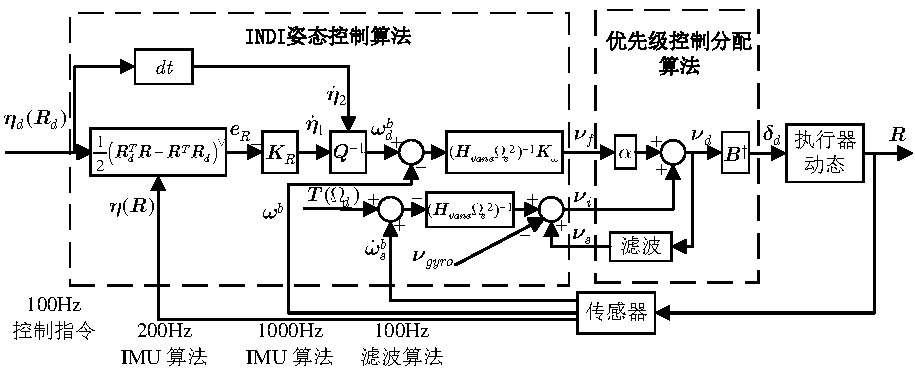
\includegraphics[scale=1]{Fig/实际框图.pdf}
		\caption{\label{实际框图}基于INDI和优先级控制分配法的姿态控制系统框图}
	\end{minipage}%
\end{figure}

\section{实验和结果分析}

为了验证提出的基于上层INDI+底层优先级控制分配的姿态控制方法的性能,本小节进行了一系列仿真实验与实际飞行实验,包括INDI姿态控制方法对比串级PID姿态控制方法和优先级控制分配方法对比伪逆方法。作为对照实验的串级PID控制方法中,角度环采用单一的P控制器,角速度环采用PI控制器。实验过程中使用的INDI姿态控制器和串级PID姿态控制器的参数如下表\ref{Control_parameters}所示,$\boldsymbol{K}_{R}$表示角度环比例增益,$\boldsymbol{K}_{\omega}$表示角速度环比例增益,$\boldsymbol{I}_{\omega}$表示角速度环积分增益。为了保证实验过程中其他条件的一致性,在INDI控制对比PID控制的实验过程中,底层控制分配方法都采用伪逆法。而在优先级控制分配方法对比伪逆方法的实验过程中,上层姿态控制均采用INDI方法。
\begin{table}
	\caption{\label{Control_parameters}INDI控制器和PID控制器的各项参数}
	\centering
	\small 
	\begin{tabular}{cccccc}
		\hline 
		INDI控制器参数符号 & 数值 & PID控制器参数符号 & 数值 & PID控制器参数符号 & 数值 \tabularnewline
		\hline 
		$K_{R\varphi}$ & $5.5$ & $K_{R\varphi}$ & $5.5 $& $I_{\omega p}$ & $0.1$ \tabularnewline
		$K_{R\theta}$   & $5.5$ & $K_{R\theta}$   & $5.5$& $I_{\omega q}$   & $0.1$ \tabularnewline
        $K_{R\psi}$   & $5.0$ & $K_{R\psi}$   & $5.0$& $I_{\omega r}$   & $0.1$ \tabularnewline
        $K_{\omega p}$   & $0.3$ & $K_{\omega p}$   & $0.3$ \tabularnewline
        $K_{\omega q}$   & $0.3$ & $K_{\omega q}$   & $0.3$ \tabularnewline
        $K_{\omega r}$   & $0.18$ & $K_{\omega r}$   & $0.18$ \tabularnewline
		\hline 
	\end{tabular}
\end{table}

仿真实验平台为MATLAB,DFUAV的仿真模型相关参数参考表\ref{DFUAV_parameters},仿真模型中采用基于龙格-库塔(Runge-Kutta)法的ode45数值求解器求解DFUAV的非线性动态方程(式\eqref{eq_10})。实际飞行实验平台使用2.1节介绍的试验样机。为了提高数据的一致性并且减少风扇转速$\Omega$变化带来的耦合效应,需要保证姿态控制过程中的高度稳定,因此实验中采用了位置控制器,该控制器的设计方法将于第四章具体介绍。应当注意的是,位置控制器的加入并不影响姿态控制器的性能验证。悬停时风扇的旋转速度约为7639转/分钟。

为了体现所提出的姿态控制器的抗干扰性能,本文设计了一种主动产生扰动的方案。由于姿态动力学系统的输入信号为控制舵面的偏转角度,所以实验中通过在一些控制舵面上添加固定的偏置来引入干扰,如图\ref{主动扰动}所示。此外,为了防止因加入固定偏置而导致控制舵面饱和的问题,当添加固定偏置时,对应控制舵面的最大偏转角度也应该同步调整。调整时也需要确保控制算法在正负方向上响应的对称性。例如在1号控制舵面上添加了$5^{\circ}$的固定偏置,那么1号控制舵面的最大偏转角度应该限制为$\pm(\delta_m-5^{\circ})$,即$\pm35^{\circ}$,其他舵面的最大偏转角度保持$\pm40^{\circ}$不变。

\begin{figure}[htbp]
	\centering
        \subfloat[INDI对比PID的扰动设置]
		{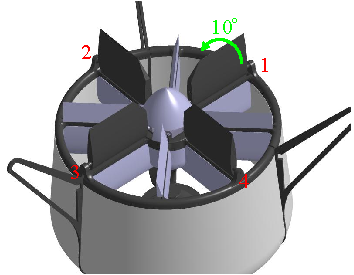
\includegraphics[scale=1]{Fig/主动扰动1.pdf}
		\label{实验一扰动}}
        \subfloat[优先级控制分配对比伪逆的扰动设置]
        {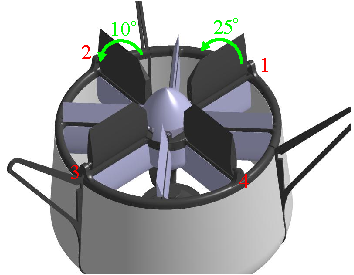
\includegraphics[scale=1]{Fig/主动扰动2.pdf}
		\label{实验二扰动}}
    \caption{主动扰动实验设置}\label{主动扰动}
\end{figure}

\subsection{仿真实验}

\subsubsection{INDI对比PID}

本实验的目的是验证在MATLAB仿真环境中搭建的INDI控制器在有无干扰情况下的性能,采用PID姿态控制器作为实验对比。扰动的添加方式如图\ref{实验一扰动}所示,在1号控制舵面上添加$10^{\circ}$的固定偏置,这会在机体上产生额外的负滚转力矩和正偏航力矩,1号舵的偏转角度限幅被同时调整为$\pm30^{\circ}$。实验总时长为6s,仿真步长为0.01s。仅在滚转通道设置方波指令信号,俯仰和偏航通道的指令均设置为0。

没有添加扰动时的实验对比结果如图\ref{INDI对比PID仿真无扰动}所示。根据实验结果可知,在滚转通道上,INDI控制和PID控制都可以及时地跟踪期望姿态指令,但是相比于PID控制,INDI控制器的超调量相对较小,并且收敛速度更快。对于俯仰和偏航通道,添加了陀螺力矩补偿的INDI控制器在滚转姿态变化时能够更好地抑制陀螺力矩的影响,从而提高了姿态控制的精度。
\begin{figure}[htbp]
	\centering
	\begin{minipage}[c]{1\textwidth}
        \centering
        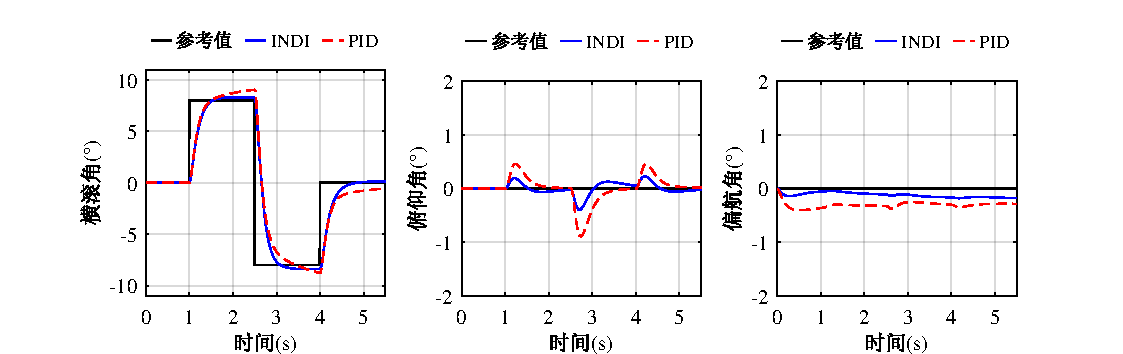
\includegraphics[scale=1]{Fig/INDI对比PID无扰动仿真实验结果.pdf}
        \caption{\label{INDI对比PID仿真无扰动}INDI对比PID在无扰动情况下的仿真实验结果}
        \end{minipage}
\end{figure}

添加干扰情况下的实验对比结果如图\ref{INDI对比PID仿真有扰动}所示,扰动在方波输入时同步添加。在滚转通道上,INDI控制器在添加扰动后仍然能够保持较好的跟踪性能,似乎与未添加扰动情况下的姿态响应曲线没有区别,这是由于INDI控制器能够补偿未建模动态力矩$\boldsymbol{M}_a^b$,并且在每一个控制周期内都会实时补偿而不会积累误差。但是PID控制器依赖误差才能修正,存在未知扰动的情况下由于无法及时预测和补偿误差,所以表现出了明显的滞后与超调量,并且在INDI控制下的姿态达到稳态时,PID控制下的姿态仍存在明显的偏差。在偏航通道上,INDI对于扰动引起的偏航力矩的抑制能力同样明显优于PID。
\begin{figure}[htbp]
	\centering
	\begin{minipage}[c]{1\textwidth}
        \centering
        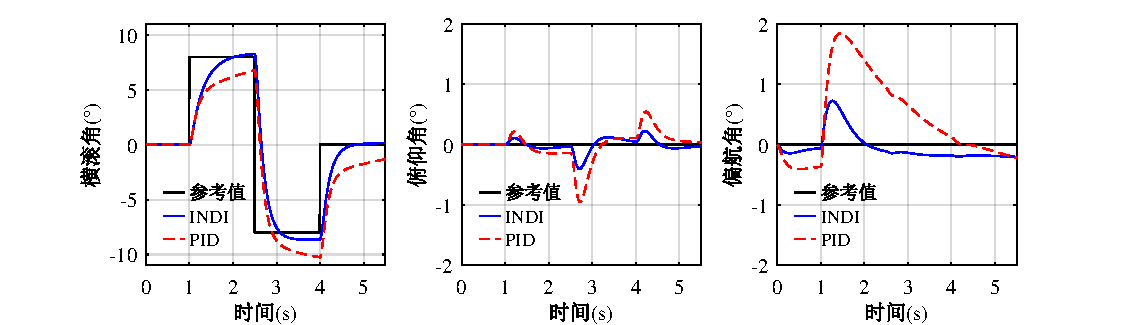
\includegraphics[scale=1]{Fig/INDI对比PID有扰动仿真实验结果.pdf}
        \caption{\label{INDI对比PID仿真有扰动}INDI对比PID在有扰动情况下的仿真实验结果}
        \end{minipage}
\end{figure}

\subsubsection{优先级控制分配对比伪逆}

本实验用于验证设计的优先级控制分配算法在控制舵面饱和情况下的有效性,对比实验为前文提到的伪逆方法。扰动的添加方式如图\ref{实验二扰动}所示,在1号控制舵面上添加$25^{\circ}$的固定偏置,并且在2号控制舵面上添加$10^{\circ}$的固定偏置,这会在机体上产生额外的负滚转力矩、负俯仰力矩和正偏航力矩。1号舵的偏转角度限幅被同时调整为$\pm15^{\circ}$,2号舵的偏转角度限幅被同时调整为$\pm30^{\circ}$。实验总时长为2s,仿真步长为0.01s。为了便于观察三个通道受扰动影响的情况,三个姿态通道的参考指令均设置为0,扰动在第1s时刻添加。

姿态通道的实验结果如图\ref{优先级伪逆姿态仿真}所示。可以看出,三个姿态通道的误差变化情况都与扰动产生的力矩的变化情况相一致。但是以优先级控制分配算法作为底层分配算法时的姿态通道误差幅值明显比伪逆法更小,这是由于优先级控制分配算法优先满足了高优先级分量$\boldsymbol{\nu}_i$,使执行机构的变化能够及时地补偿未建模动态力矩的影响。这也说明了本文的划分优先级分量思路的正确性。
\begin{figure}[htbp]
	\centering
	\begin{minipage}[c]{1\textwidth}
        \centering
        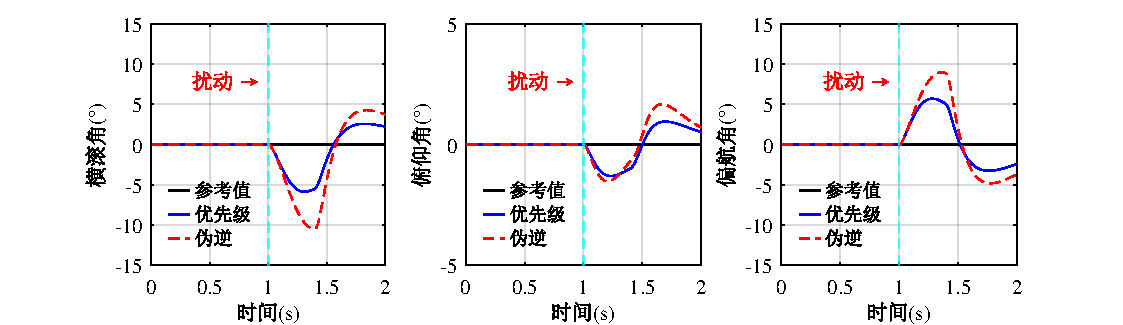
\includegraphics[scale=1]{Fig/优先级对比伪逆的姿态保持仿真实验结果.pdf}
        \caption{\label{优先级伪逆姿态仿真}优先级控制分配对比伪逆法的姿态保持仿真实验结果}
        \end{minipage}
\end{figure}

另一种可以直观感受控制分配方法优劣的方式是比较分配误差。伪逆方法的分配误差定义为:
\begin{equation}
    \boldsymbol{e}_{pinv}=\boldsymbol{\nu}_d-\boldsymbol{B}\boldsymbol{\delta}_d
    \label{3-66}
\end{equation}
其中$\boldsymbol{\delta}_d$是通过式\eqref{3-57}计算得到的,该值需要被限制在容许控制集合$\boldsymbol{U}$内。

优先级控制分配算法的分配误差定义为$\boldsymbol{e}_{i}+\boldsymbol{e}_{f}$,两个分量分别表示INDI分配误差和反馈分配误差。可以通过下式计算:
\begin{equation}
    \begin{gathered}
        \begin{cases}
            \boldsymbol{e}_{i}=\boldsymbol{\nu}_i-\boldsymbol{B}\boldsymbol{\delta}^{\prime} \\
            \boldsymbol{e}_{f}=\boldsymbol{\nu}_f-\boldsymbol{B}\boldsymbol{\delta}^{\prime\prime}
        \end{cases}
    \end{gathered}
    \label{3-67}
\end{equation}
其中$\boldsymbol{\delta}^{\prime}$可以由式\eqref{3-61}计算得到,$\boldsymbol{\delta}^{\prime\prime}$可以由式\eqref{3-63}计算得到。

两种分配方法对应的分配误差如图\ref{优先级伪逆分配误差仿真}所示。可以看出,扰动添加的瞬间立刻在三个通道上产生分配误差。但是优先级控制分配算法的分配误差在扰动添加之后的短暂时间内迅速减小,而伪逆方法的分配误差则是不断增大一段时间才减小,且分配误差的幅值也明显大于优先级控制分配算法。说明本文使用的优先级控制分配算法提高了姿态控制的精度。
\begin{figure}[htbp]
	\centering
	\begin{minipage}[c]{1\textwidth}
        \centering
        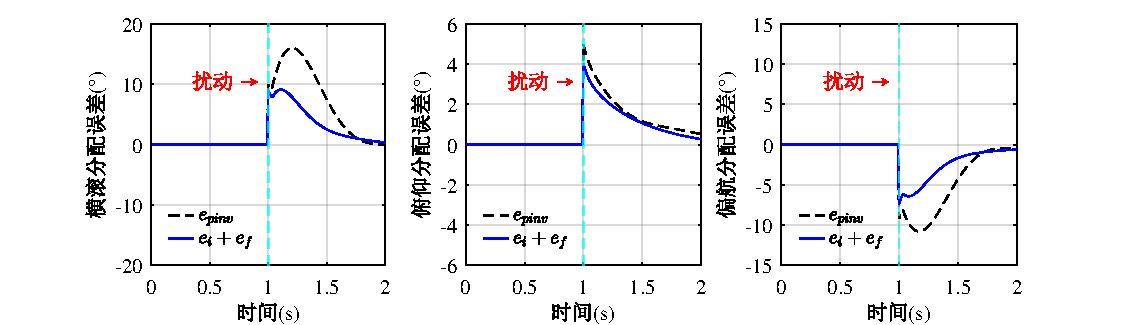
\includegraphics[scale=1]{Fig/优先级对比伪逆的分配误差仿真实验结果.pdf}
        \caption{\label{优先级伪逆分配误差仿真}优先级控制分配对比伪逆法的分配误差仿真实验结果}
        \end{minipage}
\end{figure}

图\ref{优先级分量分配误差仿真}展示了仿真实验中优先级分量各自对应的分配误差$\boldsymbol{e}_i$和$\boldsymbol{e}_f$的比较。从图中可以明显的看出INDI分配误差$\boldsymbol{e}_i$始终保持为零,这表明分量$\boldsymbol{\nu}_i$在实验过程中始终满足可达性约束,这是因为INDI输入分量位于高优先级,分配算法将优先满足该分量。而优先级控制分配的分配误差全由反馈分配误差$\boldsymbol{e}_f$贡献,这表明了优先级控制分配算法由于控制舵面的饱和对反馈输入进行了截断。通过仿真实验验证了优先级控制分配算法的可行性和有效性。
\begin{figure}[htbp]
	\centering
	\begin{minipage}[c]{1\textwidth}
        \centering
        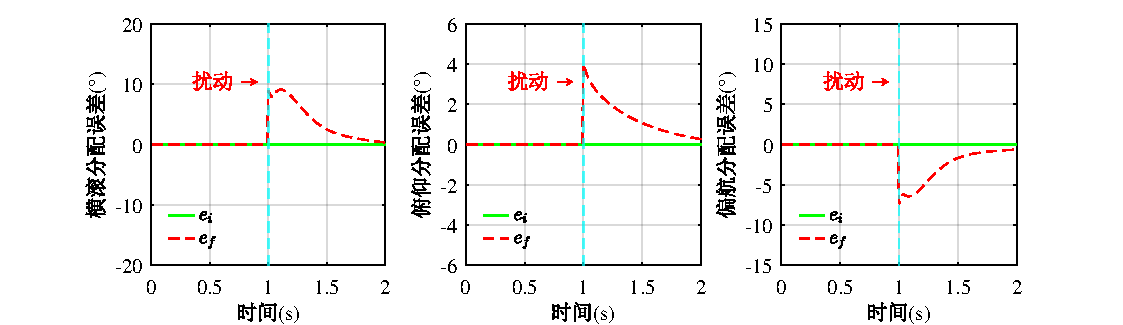
\includegraphics[scale=1]{Fig/优先级各分量的分配误差仿真实验结果.pdf}
        \caption{\label{优先级分量分配误差仿真}优先级分量各自的分配误差仿真实验结果}
        \end{minipage}
\end{figure}
\subsection{实际飞行实验}

\subsubsection{INDI对比PID}

本实验的目的是使用第二章介绍的试验样机验证提出的基于INDI的姿态控制器在实际飞行中是否能够稳定的跟踪期望姿态以及抵抗外部干扰的能力。实验过程同样分为无扰动和有扰动两种情况。实验条件的设计与仿真实验中保持一致,包括扰动的添加方式(见图\ref{实验一扰动})和方波指令的输入等。实际控制器的步长为0.01s。

无扰动和有扰动情况下的姿态控制实际飞行实验结果分别如图\ref{INDI对比PID无扰动飞行实验结果}和图\ref{INDI对比PID有扰动飞行实验结果}所示。从实验结果可以看出,在实际飞行情况下,INDI姿态控制器跟踪期望姿态的能力同样优于PID姿态控制器。相比PID,INDI在滚转通道的超调量更小,上升时间更短,在俯仰和偏航通道上的姿态误差也更小。结果与仿真实验中相符。

在添加干扰的情况下,INDI姿态控制器同样也表现出了更好的抗干扰能力,跟踪误差较小。而PID控制器则难以有效应对外部干扰,表现出了较大的跟踪误差。这进一步验证了INDI控制器在实际飞行中的有效性。
\begin{figure}[htbp]
	\centering
	\begin{minipage}[c]{1\textwidth}
        \centering
        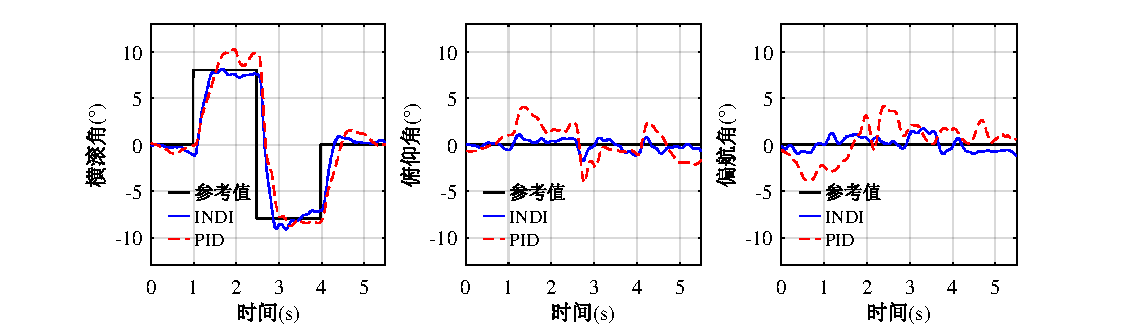
\includegraphics[scale=1]{Fig/INDI对比PID无扰动飞行实验结果.pdf}
        \caption{\label{INDI对比PID无扰动飞行实验结果}INDI对比PID无扰动时的飞行实验结果}
        \end{minipage}
\end{figure}
\begin{figure}[htbp]
	\centering
	\begin{minipage}[c]{1\textwidth}
        \centering
        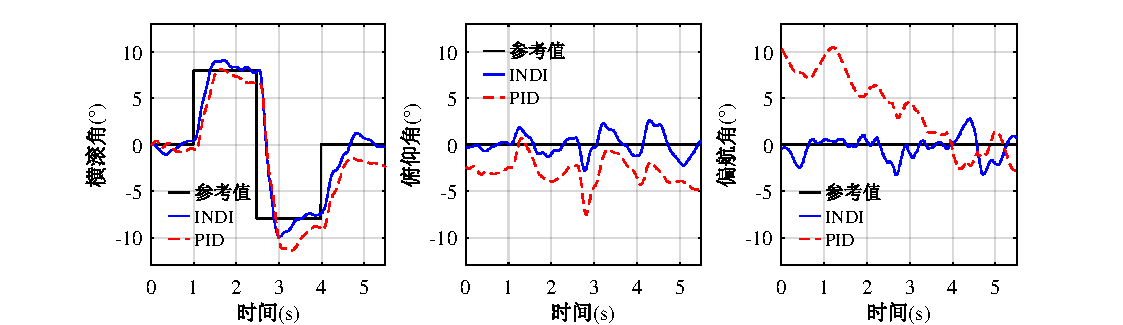
\includegraphics[scale=1]{Fig/INDI对比PID有扰动飞行实验结果.pdf}
        \caption{\label{INDI对比PID有扰动飞行实验结果}INDI对比PID有扰动时的飞行实验结果}
        \end{minipage}
\end{figure}

\subsubsection{优先级控制分配对比伪逆}

本实验用于验证设计的优先级控制分配算法在实际飞行过程中的表现情况。实验条件的设计与仿真实验中保持一致,扰动的添加方式采用图\ref{实验二扰动}中的设计,三轴期望姿态都被设置为0。对照实验采用伪逆法,两种分配算法的执行步长均为0.01s。

姿态通道的实际飞行实验结果如图\ref{优先级对比伪逆的姿态保持飞行实验结果}所示。三轴的姿态误差变化情况与主动扰动产生的力矩变化情况相一致。但是在优先级控制分配算法下,三轴姿态通道的姿态误差幅值更小,并且误差收敛的速度也更快。上述结果与仿真实验中保持一致,进一步说明了仿真实验中结果分析的正确性。
\begin{figure}[htbp]
	\centering
	\begin{minipage}[c]{1\textwidth}
        \centering
        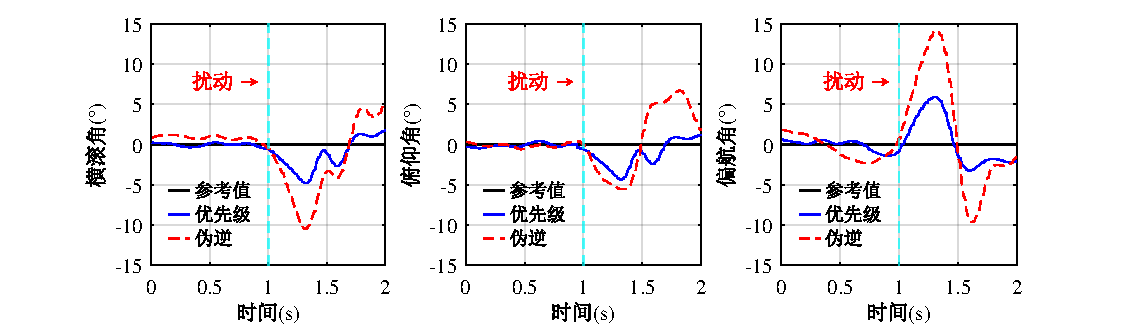
\includegraphics[scale=1]{Fig/优先级对比伪逆的姿态保持飞行实验结果.pdf}
        \caption{\label{优先级对比伪逆的姿态保持飞行实验结果}优先级对比伪逆的姿态保持飞行实验结果}
        \end{minipage}
\end{figure}

两种分配方法的分配误差的比较如图\ref{优先级对比伪逆的分配误差飞行实验结果}所示。分配误差于式\eqref{3-66}和式\eqref{3-67}中定义。从图中可以看出,伪逆方法下的总体分配误差远大于优先级控制分配算法下的分配误差,这导致了伪逆方法下的姿态误差也更大。这说明本文设计的优先级控制分配算法在实际飞行中同样能够提高姿态控制的精度。

实际飞行实验中优先级分量的分配误差比较如图\ref{优先级各分量的分配误差飞行实验结果}所示。从图中可以看出,即使是在实际飞行中,INDI输入分量$\boldsymbol{\nu}_i$也始终满足可达性约束。反馈分配误差$\boldsymbol{e}_i$的存在表明优先级控制分配算法对$\boldsymbol{\nu}_f$进行了截断。通过实际飞行实验进一步验证了优先级控制分配算法的可行性和有效性。
\begin{figure}[htbp]
	\centering
	\begin{minipage}[c]{1\textwidth}
        \centering
        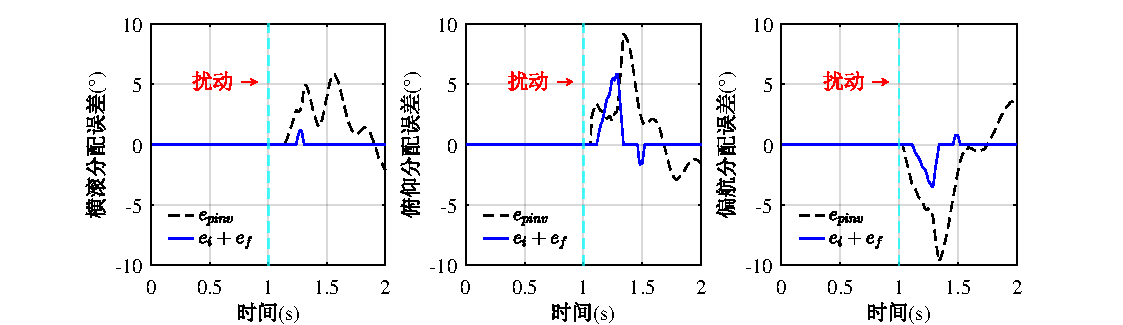
\includegraphics[scale=1]{Fig/优先级对比伪逆的分配误差飞行实验结果.pdf}
        \caption{\label{优先级对比伪逆的分配误差飞行实验结果}优先级对比伪逆的分配误差飞行实验结果}
        \end{minipage}
\end{figure}
\begin{figure}[htbp]
	\centering
	\begin{minipage}[c]{1\textwidth}
        \centering
        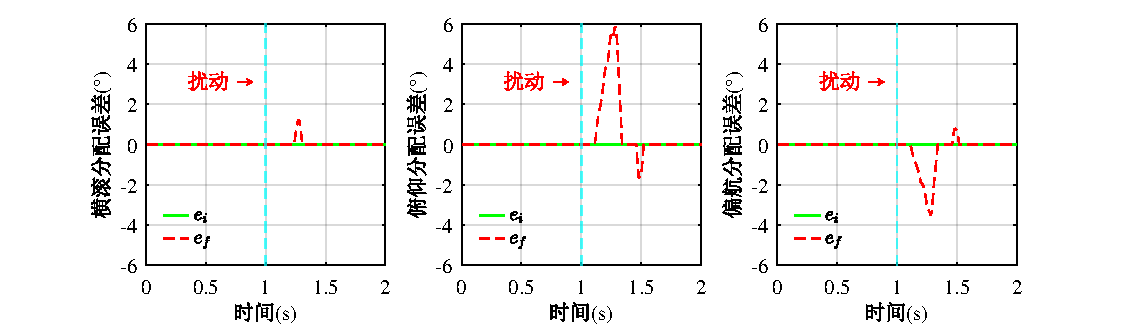
\includegraphics[scale=1]{Fig/优先级各分量的分配误差飞行实验结果.pdf}
        \caption{\label{优先级各分量的分配误差飞行实验结果}优先级各分量的分配误差飞行实验结果}
        \end{minipage}
\end{figure}

\section{本章小结}

本章围绕DFUAV的姿态控制问题展开研究,系统性地构建了基于INDI与优先级控制分配的理论框架及工程实现方案。首先介绍了INDI方法和控制分配理论以及两者在分层控制架构中的作用,然后通过姿态动力学模型简化降低了姿态动力学的非线性复杂度。进一步,提出了一种融合INDI架构与优先级控制分配的姿态控制策略,基于传感器的INDI方法对难以测得的力矩和外部扰动有较好的补偿能力,基于优先级控制分配可以最大程度保障虚拟控制输入中高优先级分量的可达性。最后通过一系列MATLAB仿真与实际飞行实验,证实了所提出的姿态控制方案相比于PID控制在扰动条件下仍能保持较小的跟踪误差,且控制分配误差也比传统的伪逆法更小。充分验证了所设计的姿态控制器的有效性,为下文的位置控制器设计奠定了基础。